% ============================================================================
%  Saussure in HLLSet Algebra --- Part I: General Principles
%  A computational exegesis of Ferdinand de Saussure's
%  Course in General Linguistics, Part One, in the Boolean lattice
%  and GF(2) ring of HLLSet Algebra
% ----------------------------------------------------------------------------
%  Series:  Saussure in HLLSet Algebra (reverse direction of influence)
%  Build:   pdflatex saussure_hllset_part1_general_principles.tex  (run twice)
%  Notation follows the EWM PUB series:
%    main.tex / companion.tex / tecs_state_machine_trajectory.tex /
%    attention_lattice_traversal.tex / langue_as_a_lattice.tex
% ============================================================================
\documentclass[11pt,a4paper]{article}

\usepackage[utf8]{inputenc}
\usepackage[T1]{fontenc}
\usepackage{amsmath,amssymb,amsthm}
\usepackage{amscd}
\usepackage{booktabs}
\usepackage{array}
\usepackage{tikz}
\usetikzlibrary{arrows.meta,positioning}
\usepackage{hyperref}
\usepackage[margin=1in]{geometry}
\usepackage{enumitem}
\usepackage{xcolor}
\definecolor{hlblue}{RGB}{0,80,160}
\hypersetup{colorlinks=true,linkcolor=hlblue,urlcolor=hlblue,citecolor=hlblue}

% ---- theorems (aligned with the PUB series) --------------------------------
\newtheorem{principle}{Principle}[section]
\newtheorem{theorem}[principle]{Theorem}
\newtheorem{definition}[principle]{Definition}
\newtheorem{proposition}[principle]{Proposition}
\newtheorem{corollary}[principle]{Corollary}
\newtheorem{remark}[principle]{Remark}
\theoremstyle{remark}
\newtheorem{observation}[principle]{Observation}
\newtheorem{reading}[principle]{Reading}

% ---- shorthands (aligned with the PUB series) ------------------------------
\newcommand{\Plane}{\ensuremath{\mathbb{B}}}            % bit plane
\newcommand{\Lat}{\ensuremath{\mathcal{B}}}              % HLLSet (Boolean) lattice
\newcommand{\Tok}{\ensuremath{\mathcal{T}}}              % token space
\newcommand{\HLL}{\ensuremath{H}}                        % an HLLSet
\newcommand{\xor}{\ensuremath{\Delta}}                   % ring addition
\newcommand{\BSS}{\ensuremath{\mathsf{BSS}}}             % BSS measure
\newcommand{\res}{\ensuremath{\mathrm{res}}}             % residual
\newcommand{\spanof}[1]{\ensuremath{\langle #1\rangle}}  % GF(2) span
\newcommand{\supp}{\ensuremath{\mathrm{supp}}}           % support
\newcommand{\Attn}{\ensuremath{\mathrm{Attn}}}           % attention operator
\newcommand{\Ctx}{\ensuremath{\mathcal{C}}}              % token context
\newcommand{\Ing}{\ensuremath{\mu}}                      % ingestion morphism
\newcommand{\Mat}{\ensuremath{\rho}}                     % materialization morphism
\newcommand{\Lang}{\ensuremath{\mathcal{L}}}             % langue (the lattice system)
\newcommand{\Par}{\ensuremath{\mathcal{P}}}              % parole (usage)
\newcommand{\Sign}{\ensuremath{\mathcal{S}}}             % the sign relation
\newcommand{\Cov}{\ensuremath{\mathrm{cov}}}             % coverage
\newcommand{\Disp}{\ensuremath{\mathcal{D}}}             % the dispatcher
\newcommand{\Sync}{\ensuremath{\mathsf{Syn}}}            % synchronic fiber
\newcommand{\Dia}{\ensuremath{\mathsf{Dia}}}             % diachronic trajectory
\newcommand{\Gen}{\ensuremath{\gamma}}                   % basis generation
\newcommand{\cover}{\ensuremath{\mathrm{cover}}}         % frame cover

% ---- title -----------------------------------------------------------------
\title{\textbf{Saussure in HLLSet Algebra}\\[4pt]
\large Part I: General Principles\\[4pt]
\large A Computational Exegesis of the \textit{Course in General Linguistics},\\
Part One, in the Boolean Lattice and GF(2) Ring of HLLSet Algebra\\[6pt]
\normalsize First paper in the series \textit{Saussure in HLLSet Algebra}}

\author{Alex Mylnikov \and Alexandr Mylnikov Jr. \and Deependra Kumar}
\date{\today}

\begin{document}
\maketitle

\begin{abstract}
The five papers of the EWM PUB series used Saussure's \textit{Course in General
Linguistics} as an interpretive lens: langue, parole, the sign, and value were
read \emph{into} the HLLSet Boolean lattice and its GF(2) ring. This paper
reverses the direction of influence. We read Saussure's text \emph{out of} the
algebra: the \textit{Course} is treated as a specification, HLLSet Algebra as
the implementation, and each principle of Part One (General Principles) is
required to hold either \emph{by construction}---as a theorem of the lattice or
the ring---or \emph{by measurement}---as a named invariant of the running
system. Part One yields the following dictionary. The linguistic sign is the
pair of a lattice node and its materialized context, connected by the two
morphisms $(\Ing,\Mat)$; the signifier is a bit-set in the one-dimensional
plane, and the signified is the node's differential value in the current frame.
Principle~I (arbitrariness of the sign) becomes a theorem of coordinate
freedom: every permutation of the plane is a simultaneous automorphism of the
Boolean lattice and the Boolean ring, so no structural property prefers one
IICA morphism over another, while idempotence, immutability, and content
addressability fix the chosen bond as the social contract. Principle~II (the
linear character of the signifier) is realized twice: as the line of bit
positions and as GF(2)-linearity of the ring basis. The chapter on immutability
and mutability is re-founded as a two-layer theorem: IICA and join-monotonicity
make the individual sign immutable, while basis generations re-coordinate the
\emph{value} of every sign, so the language changes although no speaker changes
it. The chapter on static and evolutionary linguistics becomes a fibration:
a synchronic fiber $\Sync(t)=(\Lat,F(t),\Gen(t))$ over each time step, a
diachronic trajectory $\Dia$ across fibers, lattice identities as synchronic
laws (general but not imperative), recorded transitions as diachronic laws
(imperative but not general), the Boolean ring axioms as the panchronic layer
that carries no linguistic content, and the chess analogy as the theorem that
value is frame-relative. The paper closes with the full dictionary of Part One
and a statement of what the reversal of direction changes methodologically.
\end{abstract}

\noindent\textbf{Keywords:} Saussure; Course in General Linguistics; general
principles; linguistic sign; arbitrariness; linearity; immutability;
mutability; synchrony; diachrony; panchrony; HLLSet; Boolean lattice; GF(2)
ring; IICA morphism; basis generation; computational exegesis.

% ============================================================================
\section{Introduction}
\label{sec:intro}
% ============================================================================

\subsection{The direction of influence, reversed}

In the preceding EWM series---the consolidation document, the lattice
companion, the state-machine trajectory, the attention traversal, and the
closing paper \textit{Langue as a Lattice}---Saussure's \textit{Course in
General Linguistics} \cite{saussure1916} functioned as an interpretive lens.
The \textit{Course} supplied the vocabulary (langue, parole, sign, value,
difference) through which the HLLSet Boolean lattice and its GF(2) ring were
recognized as a computable structuralism \cite{ewm2026,companion2026,state2026,attention2026,langue2026}.
The direction of influence ran from Saussure to the algebra.

This paper reverses the arrow. We no longer ask ``what does Saussure illuminate
in HLLSet Algebra?'' We ask: \textbf{what does HLLSet Algebra illuminate in
Saussure?} The \textit{Course} becomes the object of study, and the algebra
becomes the instrument of interpretation. The genre changes accordingly: this
is not an engineering paper that borrows a philosophical vocabulary, but a
\emph{computational exegesis}---a reading of Saussure's text in which every
term must receive a datatype or an operation, and every principle must receive
a theorem or an invariant.

\subsection{Method: principles as theorems, terms as datatypes}

The method has three rules, and we state them in advance because they are the
whole discipline of the series.

\begin{enumerate}[leftmargin=*,nosep]
  \item \textbf{No metaphor.} A Saussurean term is interpreted only when it has
    been assigned a concrete object of the algebra (a set, a node, a morphism,
    a frame, a measure). Until then it remains uninterpreted, and we say so.
  \item \textbf{Principles become theorems or invariants.} A Saussurean
    principle is interpreted only when it can be stated as a proposition of the
    algebra (proved from the definitions) or as an invariant of the running
    system (a quantity the algebra preserves). If neither is possible, the
    principle is recorded as a \emph{residual}: an open problem of the
    interpretation, not a victory.
  \item \textbf{Ambiguity is data.} Where the \textit{Course} is genuinely
    ambiguous, the algebra often forces a disambiguation, because a datatype
    cannot be vague in the way a philosophical term can. We record which
    disambiguation was chosen, and why the algebra demanded it.
\end{enumerate}

The method is falsifiable in a way that philosophical commentary is not: each
Reading below can be checked by running the reference implementation, and each
theorem by the usual means.

\subsection{Note on the text and the translations}

The authors' working copy of the \textit{Course} has been the Russian
translation of A.~M.~Sukhotin, as edited in \cite{saussure1977}. For this
series, aimed at an English-reading audience, we cite the English translation
of Roy Harris \cite{harris1983}, with the French original of 1916
\cite{saussure1916} as the source of record and the Russian edition retained
for the authors' verification. One terminological note is required once.
Harris renders \emph{signifiant}/\emph{signifi\'e} as
\emph{signal}/\emph{signification}; the older and now-standard English terms,
due to Baskin \cite{baskin1959}, are \emph{signifier}/\emph{signified}. We keep
the standard pair and mark the equivalence: \emph{signal} = signifier,
\emph{signification} = signified. References to the \textit{Course} are given
by part, chapter, and section rather than page numbers, so that they hold
across the French, English, and Russian editions.

\subsection{What Part One contains, and the series roadmap}

Part One of the \textit{Course}, ``General Principles,'' contains three
chapters: (I) the nature of the linguistic sign, with the two principles of
arbitrariness and linearity; (II) the immutability and mutability of the sign;
(III) static and evolutionary linguistics, with the two axes, the two kinds of
law, and the chess analogy. This paper follows the same order, after a compact
preliminary section that fixes the algebra.

The series is planned to follow the architecture of the \textit{Course} in
reverse order of dependency. Part II will treat Synchronic Linguistics (value,
``differences without positive terms,'' syntagmatic and associative relations);
Part III, Diachronic Linguistics (phonetic change and analogy as basis pivots
and generation drift); Part IV, Geographical Linguistics (dialects and
substrata as host languages, codebooks, and the dispatcher); Part V, Questions
of Retrospective Linguistics (reconstruction as time travel through old
frames). The Introduction of the \textit{Course} (langue and parole, the object
of linguistics) was already read in the EWM direction in
\cite{langue2026}; its reverse reading will be folded into Part II, where
value requires the langue/parole distinction to be re-founded from the algebra
side.

% ============================================================================
\section{Preliminaries: HLLSet Algebra in one page}
\label{sec:prelim}
% ============================================================================

The reference system is the content-addressed state machine of the EWM
programme. We recall only what Part One of the \textit{Course} needs; full
treatments are in \cite{ewm2026,companion2026,state2026,attention2026,langue2026}.

\begin{definition}[Plane, lattice, ring]
\label{def:plane}
The \textbf{plane} is the fixed set
\[
  \Plane \;=\; \{0,\dots,32767\}
\]
of $32{,}768$ bit positions. The \textbf{HLLSet lattice} is the powerset
\[
  \Lat \;=\; \mathcal{P}(\Plane),
\]
a Boolean lattice under $\cup$ (join), $\cap$ (meet), and $\subseteq$ (order),
and simultaneously a Boolean ring under $\xor$ (symmetric difference, written
$\Delta$) and $\cap$ \cite{birkhoff1940}. A node of $\Lat$ is an
\textbf{HLLSet}. Cardinalities are written $|X|$; the complement of $X$ in
$\Plane$ is $\overline{X} = \Plane \setminus X$.
\end{definition}

\begin{definition}[IICA morphism, ingestion, materialization]
\label{def:iica}
A map $\Ing : \Tok \to \Lat$ from tokens to nodes is an \textbf{IICA
morphism} if it is (i) \emph{idempotent}, read as deterministic: the same token
always maps to the same node; (ii) \emph{immutable}: once fixed, the image is
never rewritten; (iii) \emph{content-addressed}: the image is named by its
content alone. It extends to finite token sets by union:
$\Ing(X) = \bigcup_{t \in X} \Ing(\{t\})$. \textbf{Materialization}
$\Mat : \Lat \dashrightarrow \Ctx$ is the partial inverse that restores, from a
node, an ordered token context through the door \cite{attention2026}.
\end{definition}

\begin{proposition}[Ingestion is join-preserving; the morphism step]
\label{prop:join}
For finite token sets $X,Y \subseteq \Tok$,
\[
  \Ing(X \cup Y) \;=\; \Ing(X) \cup \Ing(Y).
\]
Consequently the statistics of usage (co-occurrence, overlap, containment)
reduce to one operation, union, on one shared plane; frequency and linear order
are forgotten at the door and restored, when needed, by materialization.
(Throughout this paper $\Ing$ is the flat, join-preserving IICA morphism;
the windowed $n$-gram morphism of \cite{state2026} satisfies the inclusion
form $X \subseteq Y \Rightarrow \Ing(X) \subseteq \Ing(Y)$, and the
linguistic readings below hold in the image of whichever IICA morphism is
chosen.)
\end{proposition}

\begin{definition}[BSS, document coverage, basis frames, generations]
\label{def:frame}
Against a reference node $B_w \subseteq \Plane$, the \textbf{directed soft key}
is
\[
  \BSS_w(X) \;=\; \frac{|X \cap B_w|}{|B_w|}.
\]
For a context $X$ read against a document $D$, the \textbf{document coverage
reading} is
\[
  N_D = |D \setminus X|, \qquad R_D = |D \cap X|, \qquad \Cov = R_D/|D|.
\]
A \textbf{basis frame} is a reduced (RREF) GF(2) basis $F = (B_1,\dots,B_k)$ of
a span of observed nodes; the frame is stamped with a \textbf{generation}
$\Gen$ that increments whenever the basis is recomputed. Relative to $F$, a
node $X \in \spanof{F}$ has a unique \textbf{hard key} $c \in
\mathrm{GF}(2)^k$ with
\[
  X \;=\; \bigoplus_{i : c_i = 1} B_i,
\]
the \textbf{soft key} $w_i = \BSS_{B_i}(X)$ for $i=1,\dots,k$, and the
\textbf{spill} $s = |X \setminus \cover(F)|$ measuring what the frame cannot
yet see \cite{state2026}.
\end{definition}

\begin{remark}[Permutation invariance]
\label{rem:perm}
Every invariant used in this paper---cardinalities, BSS, the document
coverage numbers, rank, spill---depends only on cardinalities of
intersections and unions.
Hence it is unchanged by any permutation of the plane. This single observation
will carry the formal reading of arbitrariness in Section~\ref{sec:ch1}.
\end{remark}

% ============================================================================
\section{Chapter I: The nature of the linguistic sign}
\label{sec:ch1}
% ============================================================================

\subsection{Sign, signifier, signified}
\label{sec:sign}

Saussure opens Part One by rejecting the nomenclature view: a language is not
``a list of terms corresponding to a list of things'' \cite[Part I, ch.~I,
\S1]{harris1983}. The linguistic sign is a \emph{two-sided psychological
entity} uniting, not a thing and a name, but a concept and a sound pattern.
The two sides are inseparable, like the two faces of a sheet of paper; and both
are psychological---the sound pattern is not the material sound but its
imprint on the speaker's mind.

The HLLSet reading drops the psychologism and keeps the structure: a sign is a
\emph{two-sided object} in which the two sides are connected by two morphisms,
not by a sheet of paper.

\begin{reading}[The linguistic sign]
\label{read:sign}
Let $A \in \Lat$ be a node, $\Ctx_A = \Mat(A)$ its materialized context, and
$X_A \subseteq \Tok$ the token content that ingests to $A$, so that
$\Ing(X_A) = A$. The \textbf{sign} is the pair
\[
  \Sign \;=\; (\Ing, \Mat),
  \qquad
  \Ing : \Ctx \to \Lat, \qquad \Mat : \Lat \dashrightarrow \Ctx,
\]
together with the two faces of any node:
\[
\begin{CD}
\Ctx @>{\Ing}>> \Lat \\
@. @VV{\Mat}V \\
@. \Ctx
\end{CD}
\]
\begin{itemize}[leftmargin=*,nosep]
  \item The \textbf{signifier} (sound pattern) is the node $A$ itself: a
    bit-set in the one-dimensional plane, a pattern in a fixed medium, exactly
    as the acoustic image is a pattern in the fixed medium of time.
  \item The \textbf{signified} (concept) is the \emph{differential value} of
    $A$: its hard key $c \in \mathrm{GF}(2)^k$ in the current frame, its
    complement $\overline{A}$, and---on the side of usage---the context
    $\Ctx_A$ that materializes from it.
  \item The \textbf{bond} between the two faces is the pair of morphisms
    $(\Ing,\Mat)$, with the round-trip guarded by coverage:
    $\Mat(\Ing(\Ctx)) = \Ctx$ up to order iff $\Cov(\Ctx; D) = 1$,
    where the coverage is read against the document $D$ from which the
    context $\Ctx$ was drawn \cite{langue2026}.
\end{itemize}
\end{reading}

Two comments on the reading. First, the signifier is assigned to the node, not
to the token, because the node is what is \emph{shared} across hosts and across
paroles; the token is the private currency of one host. Second, the signified
is assigned to the differential value, not to a ``meaning,'' because Saussure
himself defines value negatively---a sign is what the others are not---and the
algebra makes that definition executable as a coordinate vector in a basis.
Full treatment of value is the subject of Part II; here only its role as the
second face of the sign is needed.

\begin{observation}[Two-sidedness without psychologism]
Saussure's insistence that both faces are psychological becomes, in the
algebra, the statement that both faces are \emph{structural}: the signifier is
a node of the shared lattice (not the physical sound), and the signified is a
position in the frame (not a private mental content). The sheet of paper is
replaced by the requirement that the two morphisms be adjoint on the image, so
that neither face exists without the other \cite{langue2026}.
\end{observation}

\subsection{Principle I: The arbitrariness of the sign}
\label{sec:arbitrariness}

Saussure's first principle: ``The link between signifier and signified is
arbitrary'' \cite[Part I, ch.~I, \S2]{harris1983}. He immediately adds two
clarifications that the later literature often loses. First, \emph{arbitrary}
does not mean that the signifier depends on the free choice of the speaker; it
means \emph{unmotivated}: there is no natural connection between the signifier
and the signified. Second, the whole linguistic system rests on this irrational
principle, and it is precisely arbitrariness that makes the system a matter of
\emph{convention} rather than of nature.

The HLLSet reading has three layers: arbitrariness as coordinate freedom,
arbitrariness as the freedom of the morphism, and fixedness as IICA.

\begin{reading}[Arbitrariness]
\label{read:arbitrariness}
The link between signifier and signified is the IICA morphism $\Ing$ together
with its materialization inverse. The link is arbitrary in the following exact
sense: \emph{nothing in the content of a token selects its node}. The
reference implementation chooses a hash, and a seed for it, for the single
reason that it spreads values evenly over the plane; any other deterministic
content-addressed map would produce the same kind of system. The link is
\emph{unmotivated} because the Boolean algebra cannot see which map was chosen.
\end{reading}

The formal content of that Reading is a theorem.

\begin{theorem}[Arbitrariness as coordinate freedom]
\label{thm:coordinate-freedom}
Let $\pi : \Plane \to \Plane$ be any permutation of the plane, and let
\[
  \pi_* : \Lat \to \Lat, \qquad \pi_*(A) \;=\; \{\pi(i) : i \in A\}.
\]
Then $\pi_*$ is simultaneously an automorphism of the Boolean lattice
$(\Lat,\cup,\cap)$ and of the Boolean ring $(\Lat,\xor,\cap)$. Consequently no
structural property of the algebra---BSS, the coverage readings, rank, spill,
hard key cardinality---can distinguish the ingestion morphism $\Ing$ from the
re-coordinated morphism $\pi_* \circ \Ing$: every such invariant is
unchanged, provided the reference objects (the basis, the document, the
reference nodes) are re-coordinated along with the nodes, i.e.\ read through
the same relabeling of the plane.
\end{theorem}

\begin{proof}
A permutation preserves cardinality and commutes with union, intersection, and
complement: $\pi_*(A \cup B) = \pi_*(A) \cup \pi_*(B)$, and likewise for
$\cap$ and $\setminus$. Hence all cardinality-defined invariants are
preserved when their reference objects are re-coordinated too. The lattice
and ring identities are preserved because $\pi_*$ is a bijective
homomorphism. Thus the two systems, $\Ing$ and $\pi_* \circ \Ing$, are
isomorphic; the theory cannot prefer one.
\end{proof}

\begin{corollary}[Unmotivated, not undetermined]
\label{cor:fixedness}
Arbitrariness in Saussure's sense is \emph{coordinate freedom}, not
indeterminacy. The bond is unmotivated because any coordinate system works; it
is nevertheless \emph{fixed}, because a community that wishes to communicate
must share one. In the algebra, the fixedness is the IICA contract itself:
idempotence makes the bond deterministic, immutability makes it stable, and
content addressability makes it the same for every host. Arbitrary yet fixed:
coordinate freedom plus IICA.
\end{corollary}

\begin{remark}[The seed as the social contract]
The reference implementation exposes the fixedness in a concrete form: the
hash \emph{type} and its \emph{seed} are parameters of the measurement regime,
not of the lattice \cite{companion2026}. Two communities with different seeds
are two languages over the same plane; within one community, the seed is never
up for individual renegotiation. This is Saussure's ``the individual cannot
choose'' stated as an access-control property of the system.
\end{remark}

\subsection{Principle II: The linear character of the signifier}
\label{sec:linearity}

Saussure's second principle: the signifier, being auditory, unfolds in time and
therefore (a) represents a span, and (b) the span is measurable in a single
dimension---it is a line \cite[Part I, ch.~I, \S3]{harris1983}. Visual
signifiers, by contrast, can offer groupings in several dimensions at once.
The whole mechanism of language, Saussure concludes, depends on this
linearity.

The HLLSet reading realizes the line twice.

\begin{reading}[Linearity of the signifier]
\label{read:linearity}
The signifier $A \subseteq \Plane$ is a subset of the \emph{one-dimensional}
medium $\Plane = \{0,\dots,32767\}$: a line of bit positions. Ingestion takes
the temporal line of speech---the chain of signifiers in parole---and compiles
it onto this spatial line, forgetting order; materialization restores temporal
order at the door. The same object is \emph{linear} in the algebraic sense:
$\Lat$ is a vector space over $\mathrm{GF}(2)$ of dimension $|\Plane|$, and
relative to a frame $F$ every node in the span has a unique coordinate vector.
The one-dimensionality Saussure required of the signifier is therefore
realized twice: as the line of bit positions, and as GF(2)-linearity of the
ring.
\end{reading}

\begin{proposition}[The signifier is linear in two senses]
\label{prop:linearity}
(i) \emph{Medium linearity.} Every signifier is a subset of the single ordered
line $\Plane$; no signifier needs a second dimension to be written. (ii)
\emph{Algebraic linearity.} For every basis frame $F=(B_1,\dots,B_k)$ and every
node $X \in \spanof{F}$, there is a unique $c \in \mathrm{GF}(2)^k$ with
\[
  X \;=\; \bigoplus_{i : c_i = 1} B_i.
\]
The hard key $c$ is the signifier's address in the system of oppositions, and
the whole of Part Two will read value off this coordinate vector.
\end{proposition}

\begin{remark}[Why linearity matters mechanically]
Saussure's point is that linearity is what makes the signifier \emph{chainable}:
elements succeed one another, and complex signs are built by concatenation.
The algebra preserves exactly this: the GF(2) span builds complex nodes by
linear combination of basis vectors, and materialization returns the chain. The
one thing the lattice forgets---linear \emph{order}---is the one thing the
door restores, which is why the sign relation needs both morphisms and not one
\cite{attention2026}.
\end{remark}

% ============================================================================
\section{Chapter II: Immutability and mutability of the sign}
\label{sec:ch2}
% ============================================================================

Chapter II of Part One states an apparent paradox: the sign is at once
\emph{immutable}---the community cannot change it---and \emph{mutable}---time
changes it continuously. Saussure gives four reasons for immutability, then
derives mutability from the same principle of arbitrariness that seemed to
guarantee immutability. The algebra resolves the paradox by separating two
layers that the text keeps fused.

\subsection{Immutability}
\label{sec:immutability}

The signifier ``is imposed rather than freely chosen''; ``the community itself
cannot control so much as a single word; it is bound to the existing language''
\cite[Part I, ch.~II, \S2]{harris1983}. Saussure's four reasons are: (1) the
arbitrariness of the sign, which gives no rational ground for preferring one
signifier over another; (2) the multiplicity of signs necessary for any
language; (3) the complexity of the system; (4) collective inertia toward
innovation.

\begin{reading}[Immutability]
\label{read:immutability}
Immutability is the IICA contract, read at the level of the stored node. No
operation of the system rewrites a node once written: ingestion is union, the
commit store appends, and the lattice has no deletion primitive. The four
Saussurean reasons map as follows.
\end{reading}

\begin{proposition}[Join monotonicity; no deletion]
\label{prop:inertia}
Every operation that writes the plane is a join. For all $A, B \in \Lat$,
\[
  A \;\subseteq\; A \cup B,
\]
so no legal write removes a bit once it is set. Individual and community alike
can only \emph{accumulate} and \emph{re-frame}; neither can rewrite a single
stored sign. Collective inertia is a theorem of the algebra, not a sociological
hope.
\end{proposition}

\begin{table}[htbp]
\centering
\begin{tabular}{@{}>{\raggedright\arraybackslash}p{4.6cm}
                    >{\raggedright\arraybackslash}p{10.6cm}@{}}
\toprule
Saussure's reason for immutability & HLLSet counterpart \\
\midrule
(1) Arbitrariness gives no rational ground for preferring another signifier &
Theorem~\ref{thm:coordinate-freedom}: any re-coordination is isomorphic,
so no node is a ``better'' name than another; there is nothing to optimize and
therefore no individual reason to change \\
(2) Multiplicity of signs &
$|\Lat| = 2^{32{,}768}$ nodes; the system is too large for any speaker to
re-coordinate, and every re-coordination would have to be global to be
consistent \\
(3) Complexity of the system &
the frame: changing one coordinate (one basis pivot) re-values all nodes
(generation increment), so the cost of change is systemic, not local \\
(4) Collective inertia &
Proposition~\ref{prop:inertia}: joins only add; the stored plane is
append-only; inertia is monotonicity \\
\bottomrule
\end{tabular}
\caption{The four Saussurean reasons for immutability, re-founded in the algebra.}
\label{tab:immutability}
\end{table}

\subsection{Mutability}
\label{sec:mutability}

``Time changes all things; there is no reason why language should escape this
universal law'' \cite[Part I, ch.~II, \S3]{harris1983}. The signifier and the
signified shift their relationship: a language ``is radically defenceless
against the factors which constantly tend to shift the relationship'' between
the two faces, and this, Saussure adds, is a consequence of the very
arbitrariness of the sign. Crucially, the shift is not made by speakers: ``the
language changes, but the speakers do not change it.''

\begin{reading}[Mutability]
\label{read:mutability}
Mutability is the \emph{generation mechanism} of the basis frames. The IICA
bond $(\Ing,\Mat)$ is fixed, but the frame around every sign---the system of
oppositions that gives the sign its value---is recomputed when the spill of new
observations demands it. The value of each sign changes; the sign itself, as a
stored node and as a content-addressable bond, does not.
\end{reading}

\begin{proposition}[Mutability as generation change]
\label{prop:mutability}
Let $F$ be a basis frame with generation $\Gen$, and let a new observation
$Y$ arrive whose residual against $F$ is non-empty, $\res_F(Y) \neq
\varnothing$ (in particular, this holds when the spill
$s = |Y \setminus \cover(F)|$ is positive). Recomputing the RREF
basis produces a new frame $F'$ with generation $\Gen+1$. For an unchanged
node $X \in \spanof{F}$, the hard key generally changes, $c \mapsto c'$,
although $X$ itself is untouched (IICA) and its content is untouched
(content addressability). The \emph{value} of the sign has changed while the
\emph{sign} has not.
\end{proposition}

\subsection{The paradox resolved: two layers}
\label{sec:paradox}

\begin{observation}[Immutability and mutability live on different layers]
\label{obs:two-layers}
Saussure's text states both properties of the sign without separating the
layers on which they operate. The algebra forces the separation, and the
paradox dissolves:
\begin{enumerate}[leftmargin=*,nosep]
  \item \textbf{The contract layer} (IICA: the morphism $\Ing$, the stored
    node, the content-addressable bond) is immutable---by construction, by
    Proposition~\ref{prop:inertia}.
  \item \textbf{The value layer} (the frame $F(t)$, the generation $\Gen(t)$,
    the hard and soft keys, the materialization door of each host) is
    mutable---by construction, by Proposition~\ref{prop:mutability}.
\end{enumerate}
``The language changes although the speakers cannot change it'' is then not a
paradox but a type distinction: speakers can write only to the contract layer
(by joining tokens), never to a node directly; the value layer changes globally
whenever the frame pivots, and it is precisely this global, uncommanded change
that is experienced as the drift of the language.
\end{observation}

\begin{remark}[The defencelessness of the system]
Saussure's ``radically defenceless'' now has a precise sense. The system has
no guard that prevents the frame from pivoting, because the pivot is the
normal response to spill---it is how the system learns. Defencelessness against
diachronic drift is the price of openness to novelty; both are the same
generation mechanism \cite{state2026}.
\end{remark}

% ============================================================================
\section{Chapter III: Static and evolutionary linguistics}
\label{sec:ch3}
% ============================================================================

\subsection{The two axes}
\label{sec:axes}

Saussure distinguishes two axes of study. The \emph{axis of simultaneities}
(AB) concerns relations among coexisting terms, excluding time; the \emph{axis
of successions} (CD) concerns the same terms together with their changes, one
at a time \cite[Part I, ch.~III, \S1]{harris1983}. The distinction is
``absolute and allows no compromise'': synchronic linguistics deals with
systems, diachronic linguistics with isolated events.

\begin{reading}[The two axes]
\label{read:axes}
The axis of simultaneities is a \emph{fiber} of the system at one time; the
axis of successions is the \emph{trajectory} across fibers.
\end{reading}

\begin{definition}[Synchronic fiber and diachronic trajectory]
\label{def:syn-dia}
Fix a time $t$ and a basis frame $F(t)$ of generation $\Gen(t)$. The
\textbf{synchronic structure} at $t$ is the fiber
\[
  \Sync(t) \;=\; (\Lat, F(t), \Gen(t)),
\]
the Boolean lattice together with its current frame: all nodes, their hard and
soft keys, containment, complement, and the BSS readings among coexisting
nodes. The \textbf{diachronic structure} is the indexed family
\[
  \Dia \;=\; \{\Sync(t) : t \in T\}
\]
together with the recorded transitions---commits, departed/retained/new
sets, generation increments---between consecutive fibers.
\end{definition}

\begin{figure}[htbp]
\centering
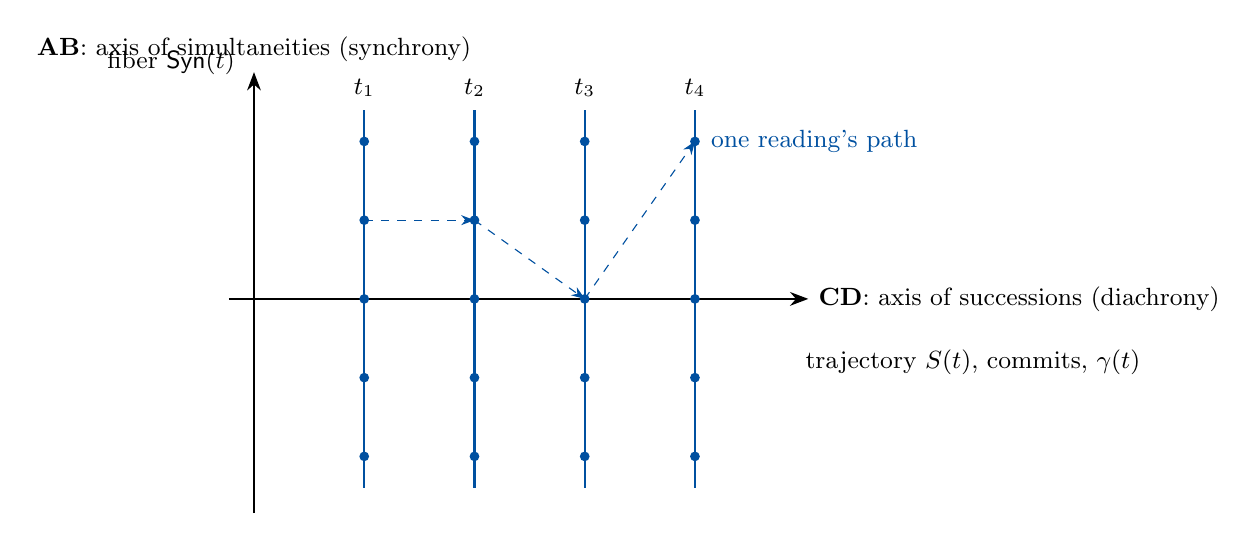
\begin{tikzpicture}[>=Stealth, scale=0.80, every node/.style={font=\small}]
  \draw[->,thick] (0,-3.4) -- (0,3.6)
    node[above] {\textbf{AB}: axis of simultaneities (synchrony)};
  \draw[->,thick] (-0.4,0) -- (8.8,0)
    node[right] {\textbf{CD}: axis of successions (diachrony)};
  \foreach \t in {1,2,3,4} {
    \draw[hlblue, thick] (\t*1.75,-3.0) -- (\t*1.75,3.0);
    \node at (\t*1.75, 3.35) {$t_{\t}$};
    \foreach \s in {-2.5,-1.25,0,1.25,2.5} {
      \fill[hlblue] (\t*1.75, \s) circle (2.2pt);
    }
  }
  \node[anchor=west] at (8.6,-1.0) {trajectory $S(t)$, commits, $\Gen(t)$};
  \node[anchor=south east] at (-0.15,3.4) {fiber $\Sync(t)$};
  \draw[->,hlblue,dashed] (1.75,1.25) -- (3.5,1.25);
  \draw[->,hlblue,dashed] (3.5,1.25) -- (5.25,0.0);
  \draw[->,hlblue,dashed] (5.25,0.0) -- (7.0,2.5);
  \node[anchor=west,hlblue] at (7.1,2.5) {one reading's path};
\end{tikzpicture}
\caption{The two Saussurean axes as a fibration: each vertical fiber
$\Sync(t)$ is a synchronic system (coexisting nodes, one frame, one
generation); the dashed path is a diachronic reading across fibers.}
\label{fig:axes}
\end{figure}

\subsection{The two kinds of law}
\label{sec:laws}

Saussure's sharpest formulation in Chapter III is the asymmetry between the two
kinds of law: a \emph{synchronic} law is \emph{general but not imperative}; a
\emph{diachronic} law is \emph{imperative but not general}
\cite[Part I, ch.~III, \S3]{harris1983}.

\begin{theorem}[The two kinds of law, re-founded]
\label{thm:laws}
(i) \emph{Synchronic laws} are the identities of the Boolean lattice and ring
in a fixed fiber $\Sync(t)$: for all nodes $A,B,C$ of the fiber,
\[
  A \cup (B \cap C) = (A \cup B) \cap (A \cup C),
  \qquad
  A \xor A = \varnothing,
  \qquad
  \Cov(X) \in [0,1],
\]
together with the uniqueness of the hard key in the frame. These hold for
\emph{every} node of the fiber---general---but they force no particular state
to occur---not imperative.
(ii) \emph{Diachronic laws} are the recorded transitions: the commit
$S(t) \to S(t+1)$ with its new and retained sets
$N = S(t{+}1) \setminus S(t)$ and $R = S(t{+}1) \cap S(t)$, the pivot
$F \to F'$, the generation increment $\Gen \to \Gen+1$. Each is
\emph{imperative}---it happened, and the commit DAG records it---but
\emph{not general}---no identity forces it, and it holds of that transition
alone.
\end{theorem}

\subsection{Panchronicity, and Saussure's warning}
\label{sec:panchrony}

Saussure considers a third possibility, the \emph{panchronic} viewpoint:
general principles that hold independently of concrete facts. His warning is
that panchronic facts, precisely because they are independent of concrete
languages, never get to grips with the specific facts of any language
\cite[Part I, ch.~III, \S4]{harris1983}.

\begin{observation}[The panchronic layer is the ring axioms]
\label{obs:panchronic}
The Boolean ring axioms are as follows: commutativity and associativity of
both operations, distributivity of $\cap$ over $\xor$, idempotence
\[
  A \cap A = A,
\]
and characteristic two
\[
  A \xor A = \varnothing.
\]
They hold in every fiber, in every generation, for every host
language. They are the panchronic layer of the system. Saussure's warning
translates exactly: these axioms are \emph{true of everything} and therefore
say nothing about any particular linguistic fact. The moment one asks a
linguistic question---what is the value of this sign? how did this form
change?---one leaves the panchronic layer and enters a fiber or a transition.
The exegesis is faithful in this precise sense: it locates Saussure's
panchronicity, not as an afterthought, but as the axioms of the algebra.
\end{observation}

\subsection{The chess analogy}
\label{sec:chess}

Saussure's comparison: a game of chess is an artificial realization of what
language presents in a natural form. A position is a synchronic state; a move
is a diachronic event; and ``the value of the pieces depends on their position
on the chessboard, just as in the language each term has its value through its
opposition to all the other terms'' \cite[Part I, ch.~III, \S5]{harris1983}.
A move changes one piece, yet it can revolutionize the whole position; in
language, likewise, a change is local but its consequences are systemic.

\begin{reading}[The chess analogy]
\label{read:chess}
The board is the plane; a position is a synchronic fiber; a move is a commit.
\end{reading}

\begin{table}[htbp]
\centering
\begin{tabular}{@{}>{\raggedright\arraybackslash}p{4.2cm}
                    >{\raggedright\arraybackslash}p{5.0cm}
                    >{\raggedright\arraybackslash}p{5.8cm}@{}}
\toprule
Chess (Saussure) & Language (Saussure) & HLLSet Algebra \\
\midrule
the board & the language as a system & the plane $\Plane$, fixed and shared \\
a position & a synchronic state & the fiber $\Sync(t) = (\Lat, F(t), \Gen(t))$ \\
the value of a piece depends on its position & the value of a term depends on its oppositions & the hard key $c$ and soft keys $w_i$ relative to $F(t)$ \\
a move changes one piece & a change is local & one commit; one token event joins one node \\
a move can revolutionize the whole position & a change has systemic consequences & a basis pivot increments $\Gen$ and re-coordinates every cached reading \cite{state2026} \\
the laws of chess outlive all games & panchronic principles & the Boolean ring axioms (Observation~\ref{obs:panchronic}) \\
\bottomrule
\end{tabular}
\caption{The chess analogy, completed by the algebra.}
\label{tab:chess}
\end{table}

\begin{remark}[Why the analogy is exact, not illustrative]
In chess the value of a piece is not written on the piece; it is computed from
the position. In HLLSet Algebra the value of a node is not written on the
node; it is computed from the frame. The algebra is the first setting in which
Saussure's analogy stops being an analogy and becomes the definition of a
datatype: value is a function of (node, frame), and nothing else.
\end{remark}

% ============================================================================
\section{The dictionary of Part One}
\label{sec:dictionary}
% ============================================================================

Table~\ref{tab:dictionary} collects the complete dictionary of Part One. Each
row is either a theorem, a proposition, or a definition of this paper; nothing
in the table is left as a suggestive parallel.

\begin{table}[htbp]
\centering
\renewcommand{\arraystretch}{1.15}
\begin{tabular}{@{}>{\raggedright\arraybackslash}p{3.6cm}
                    >{\raggedright\arraybackslash}p{4.6cm}
                    >{\raggedright\arraybackslash}p{6.8cm}@{}}
\toprule
Saussure (Part One) & In the \textit{Course} & In HLLSet Algebra \\
\midrule
linguistic sign & two-sided psychological entity & $(\Ing,\Mat)$ with faces
(node, value): Definition~\ref{def:iica}, Reading~\ref{read:sign} \\
signifier (sound pattern) & the acoustic image & the node $A \subseteq \Plane$:
a bit-set on the one-dimensional line \\
signified (concept) & the concept & the differential value: hard key $c$,
complement $\overline{A}$, materialized context \\
bond between the faces & the arbitrary link & the morphism pair
$(\Ing,\Mat)$; round-trip guarded by coverage \\
Principle I: arbitrariness & unmotivated, yet conventional & Theorem~\ref{thm:coordinate-freedom}
(coordinate freedom); Corollary~\ref{cor:fixedness} (fixed by IICA) \\
Principle II: linearity & the signifier is a line in time & Proposition~\ref{prop:linearity}:
medium line + GF(2)-linearity \\
immutability of the sign & the community cannot change it & Proposition~\ref{prop:inertia}
(join monotonicity; no deletion); Table~\ref{tab:immutability} \\
mutability of the sign & time shifts the sign & Proposition~\ref{prop:mutability}
(generation change); Observation~\ref{obs:two-layers} (two layers) \\
axis of simultaneities & AB: coexisting terms & the fiber $\Sync(t)$,
Definition~\ref{def:syn-dia} \\
axis of successions & CD: terms and their changes & the trajectory $\Dia$ and
the commit DAG, Definition~\ref{def:syn-dia} \\
synchronic law & general but not imperative & lattice/ring identities in a
fiber, Theorem~\ref{thm:laws}(i) \\
diachronic law & imperative but not general & recorded transitions,
Theorem~\ref{thm:laws}(ii) \\
panchronic viewpoint & general, independent of facts & the Boolean ring axioms,
Observation~\ref{obs:panchronic} \\
chess analogy & value depends on position & value as a function of
(node, frame), Table~\ref{tab:chess} \\
\bottomrule
\end{tabular}
\caption{The complete dictionary of Part One of the \textit{Course} into
HLLSet Algebra.}
\label{tab:dictionary}
\end{table}

% ============================================================================
\section{What the reversal changes}
\label{sec:reversal}
% ============================================================================

The five EWM papers read Saussure into the algebra; this paper reads the
algebra into Saussure. The reversal is not a symmetry of exposition. It changes
five things.

\begin{enumerate}[leftmargin=*,nosep]
  \item \textbf{From analogy to construction.} In the EWM direction, Saussurean
    terms were lenses: they helped \emph{see} the algebra as linguistics. In
    the reverse direction, the terms are \emph{requirements}: the algebra must
    satisfy them or fail. Part One satisfies them: every principle above is a
    theorem or an invariant.
  \item \textbf{Ambiguity becomes a type error.} Philosophical commentary can
    live with the ambiguity between the two layers of immutability/mutability.
    A datatype cannot. The algebra forces Observation~\ref{obs:two-layers}, and
    the forced distinction is arguably what Saussure's text was reaching for.
  \item \textbf{The text becomes testable.} Each Reading can be checked by
    running the reference implementation: ingest a corpus, pivot a frame, and
    verify that stored nodes are untouched while hard keys change. The exegesis
    is falsifiable in the laboratory, not only in the seminar.
  \item \textbf{The direction of verification reverses.} Previously Saussure
    validated the EWM programme; the risk was that the \textit{Course} was being
    used decoratively. Now the EWM programme validates Saussure; the risk is
    the opposite one, that the algebra is being used to settle questions the
    text deliberately left open. We therefore record, at each step, whether the
    algebra \emph{satisfies} a principle or \emph{disambiguates} it.
  \item \textbf{A residual is a finding, not a failure.} Where the algebra has
    no counterpart for a Saussurean claim, that is itself a result: it locates
    the claim outside the computable core. Part One leaves, so far, one such
    residual: the psychological character of the two faces, which we replaced by
    structural two-sidedness without pretending the replacement is lossless.
\end{enumerate}

% ============================================================================
\section{Conclusion and outlook to Part II}
\label{sec:conclusion}
% ============================================================================

Part One of the \textit{Course in General Linguistics} has been re-founded, in
the reverse direction, as a sequence of definitions, theorems, and invariants
of HLLSet Algebra. The sign is $(\Ing,\Mat)$; arbitrariness is coordinate
freedom; linearity is the double line of bit positions and GF(2)-span;
immutability is join monotonicity; mutability is generation change; synchrony
is a fiber, diachrony a trajectory, panchrony the ring axioms; and the chess
analogy is the definition of value as a function of (node, frame). Nothing in
the reading is a metaphor, and everything is checkable against the running
system.

Part II will take up where Part One deliberately stops: the differential theory
of value. Saussure's ``in the language itself there are only differences
without positive terms'' will be read as the statement that the value of a
node is its hard key in the current frame, that the frame itself is a system of
distinctive oppositions, and that the two axes of Part One---simultaneities and
successions---become, in Part Two, the paradigmatic and syntagmatic relations
of the lattice. The reversal of direction will then be complete in both
directions: the \textit{Course} interpreted by the algebra, and the algebra
interpreted by the \textit{Course}, as two readings of one construction.

\section*{Acknowledgments}
This paper was created in collaboration with, and with the assistance of, an
AI system---DeepSeek (deepseek-v4-pro). The computational exegesis method, the
two-layer resolution of immutability and mutability, and several of the
formulations emerged in dialogue with the assistant, whose drafts the authors
revised and take full responsibility for in their final form.

\begin{thebibliography}{99}

\bibitem{saussure1916} F.~de Saussure,
\textit{Cours de linguistique g\'en\'erale}, Payot, Paris, 1916.
(Edited posthumously by C.~Bally and A.~Sechehaye, with A.~Riedlinger.)

\bibitem{harris1983} F.~de Saussure,
\textit{Course in General Linguistics}, translated and annotated by
Roy Harris, Duckworth, London, 1983.

\bibitem{baskin1959} F.~de Saussure,
\textit{Course in General Linguistics}, translated by Wade Baskin,
Philosophical Library, New York, 1959.

\bibitem{saussure1977} F.~de Sossyur,
\textit{Trudy po yazykoznaniyu} [Works in Linguistics], edited by
A.~A.~Kholodovich, translation of the \textit{Cours} by A.~M.~Sukhotin,
Progress, Moscow, 1977.
(Authors' working copy; used for verification of the readings.)

\bibitem{ewm2026} A.~Mylnikov, A.~Mylnikov Jr., and D.~Kumar,
\textit{Emerging World Models: A Structural Framework for Self-Organizing
World Representations}, EWM PUB series, 2026.

\bibitem{companion2026} A.~Mylnikov, A.~Mylnikov Jr., and D.~Kumar,
\textit{The EWM Lattice and Its Worlds}, EWM PUB series, 2026.

\bibitem{state2026} A.~Mylnikov, A.~Mylnikov Jr., and D.~Kumar,
\textit{Transformations and Trajectories of a Content-Addressed State
Machine}, EWM PUB series, 2026.

\bibitem{attention2026} A.~Mylnikov, A.~Mylnikov Jr., and D.~Kumar,
\textit{Attention on Lattice Traversal Is All You Need}, EWM PUB series, 2026.

\bibitem{langue2026} A.~Mylnikov, A.~Mylnikov Jr., and D.~Kumar,
\textit{Langue as a Lattice: Closing the Circle from Statistical to
Structural Linguistics through Content-Addressed Algebras}, EWM PUB series,
2026.

\bibitem{birkhoff1940} G.~Birkhoff,
\textit{Lattice Theory}, American Mathematical Society, 1940.

\bibitem{maclane1971} S.~Mac Lane,
\textit{Categories for the Working Mathematician}, Springer, 1971.

\bibitem{hjelmslev1961} L.~Hjelmslev,
\textit{Prolegomena to a Theory of Language}, University of Wisconsin Press,
1961.

\bibitem{harris1954} Z.~S.~Harris,
\textit{Distributional Structure}, Word, 10(2--3):146--162, 1954.

\bibitem{firth1957} J.~R.~Firth,
\textit{A Synopsis of Linguistic Theory, 1930--1955}, Studies in Linguistic
Analysis, 1957.

\bibitem{vaswani2017} A.~Vaswani, N.~Shazeer, N.~Parmar, J.~Uszkoreit,
L.~Jones, A.~N.~Gomez, \L.~Kaiser, and I.~Polosukhin,
\textit{Attention Is All You Need}, NeurIPS, 2017.

\end{thebibliography}

\end{document}
